\documentclass{standalone}

\usepackage{tikz,siunitx}

\begin{document}
\usetikzlibrary{math} %needed tikz library
\tikzmath{\n3=5;  \n2=2; }
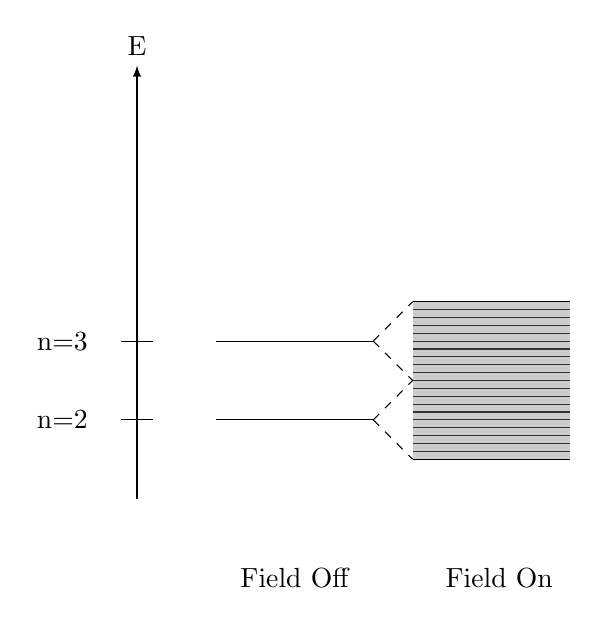
\begin{tikzpicture}[]
    \draw [-latex] (0,1) -- (0,6.5) node [above] {E};
    \draw [-] (-0.2,\n2) -- (+0.2,\n2) node [left=2em] {n=2};
    \draw [-] (-0.2,\n3) -- (+0.2,\n3) node [left=2em] {n=3};
    \draw [-] (1,\n3) -- (3,\n3);
    \draw [-] (1,\n2) -- (3,\n2);
    \draw [-,dashed] (3,\n3) -- (3.5,\n3+0.5);
    \draw [-,dashed] (3,\n3) -- (3.5,\n3-0.5);
    \draw [-,dashed] (3,\n2) -- (3.5,\n2+0.5);
    \draw [-,dashed] (3,\n2) -- (3.5,\n2-0.5);
    \node at (2.0,0) {Field Off};
    \node at (4.6,0) {Field On};
    \begin{scope}[thin]
    \foreach \y in {\n3+0.5,\n3+0.5-0.1,\n3+0.5-0.2,\n3+0.5-0.3,\n3+0.5-0.4,\n3+0.5-0.5,\n3+0.5-0.6,\n3+0.5-0.7,\n3+0.5-0.8,\n3+0.5-0.9,\n3-0.5}
    \draw(3.5,\y) -- (5.5,\y);

    \foreach \y in {\n2+0.5,\n2+0.5-0.1,\n2+0.5-0.2,\n2+0.5-0.3,\n2+0.5-0.4,\n2+0.5-0.5,\n2+0.5-0.6,\n2+0.5-0.7,\n2+0.5-0.8,\n2+0.5-0.9,\n2-0.5}
    \draw(3.5,\y) -- (5.5,\y);
    \end{scope}
    \fill [gray,opacity=0.4] (3.5,\n2-0.5) rectangle (5.5,\n2+0.5);
    \fill [gray,opacity=0.4] (3.5,\n3-0.5) rectangle (5.5,\n3+0.5);
\end{tikzpicture}
\end{document}
